\documentclass[margin=5mm, varwidth]{standalone}
\usepackage[paperwidth=9in,top=1in,bottom=1in,right=1in,left=1in,heightrounded]{geometry}
\usepackage{niftydiags}

\begin{document}
\begin{pycode}
import numpy as np
def rad(deg):
    return deg * np.pi / 180
def roundCoord(point):
    return [ round(x, 2) for x in point ]
def tuplefy(points):
    return ( tuple(roundCoord(p)) for p in points)
\end{pycode}

\section{Orthogonal complement of a vector ($90^\circ$ Rotation CCW)}
{ \large
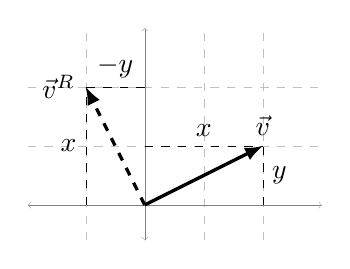
\begin{tikzpicture}[scale=1.5, ultra thin]
\draw[step=0.5cm, dashed, lightgray] (-.99,-0.3) grid (1.49, 1.49);
\draw[<->, gray] (0, -0.3) -- (0, 1.5cm);
\draw[<->, gray] (-0.99, 0) -- (1.5cm, 0);
\draw[very thick, -latex] (0, 0) -- (1, 0.5) node[above] {$\vec{v}$};% = \begin{pmatrix} x \\ y\end{pmatrix}$};
\draw[dashed] (0, .5) -- (1, .5) node[midway, above] {$x$};
\draw[dashed] (1, 0) -- (1, .5) node[midway, right] {$y$};
\draw[very thick, dashed, -latex] (0, 0) -- (-0.5, 1) node[left] {$\vec{v}^{R}$};
\draw[dashed] (0, 1) -- (-.5, 1) node[midway, above] {$-y$};
\draw[dashed] (-.5, 0) -- (-.5, 1) node[midway, left] {$x$};
\end{tikzpicture} }
$\vec{v}^{R} =  \vektor{x\\y} ^{R} = \vektor{-y\\x}$
\\
\items{
\item $\gleichung{
    \vec{v}^{R}&=&  \vektor{x \\ y} ^{R}= \vektor{\cos(\alpha) \\ \sin(\alpha)} ^{R}=\vektor{ \cos(\alpha + 90^\circ) \\ \sin(\alpha + 90^\circ) }
    \\
    &=& \vektor{ \cos(\alpha) \cos(90^\circ) - \sin(\alpha) \sin(90^\circ)  \\ \cos(\alpha) \sin(90^\circ) + \sin(\alpha) \cos(90^\circ) }
    \\
    &=&\vektor{ \cos(\alpha) \cdot 0 - \sin(\alpha) \cdot 1   \\ \cos(\alpha) \cdot 1 + \sin(\alpha) \cdot 0 }
    = \vektor{ - \sin(\alpha) \\ \cos(\alpha) } = \underline{\vektor{- y \\ x }}
}$
\item $\vec{v}^{R}$ is perpendicular to $\vec{v}$: $ \vektor{x \\ y} \bullet \vektor{-y \\ x} = \underline{-xy + yx = 0}$
}

 
\section{vector components as linear combinations of vectors} 

\items{
\item Every vector can be written as a combination of scalars and unit vectors
\item $\vec{v} = \vektor{x\\y} = x \cdot \vektor{1\\0} + y \cdot \vektor{0\\1}$
\item Generally: $\vec{v} = \vektor{x_1 \\ x_2 \\ \vdots \\ x_n} = \sum\limits_{i=1}^{n}{x_i \cdot e_i}$
\item Points on the unit cirlce: $\vec{v} = \vektor{\cos(\theta)\\ \sin(\theta)} = \cos(\theta) \cdot \vektor{1\\0} +\sin(\theta) \cdot \vektor{0\\1} = \cos(\theta) \cdot \hat{e}_1 +\sin(\theta) \cdot \hat{e}_2$
}

\section{From 2D vector arithmetic to 2D rotation matrix}

\begin{pycode}
deg=25
rotdeg=45
v=(np.cos(rad(deg)), np.sin(rad(deg)) )
v2=(-v[1],v[0])
a=np.multiply(np.cos(rad(rotdeg)), v)
b=np.multiply(np.sin(rad(rotdeg)), v2)
v3=a+b
alphaLoc = np.multiply(0.3, ( np.cos(rad(deg+rotdeg/2)), np.sin(rad(deg+rotdeg/2)) ) )
a, b, v3, alphaLoc = tuplefy([a, b, v3, alphaLoc])
\end{pycode}
\newcommand\lenax{1.2}
\begin{pysub}
    \begin{tikzpicture}[scale=2]
        \coordinate (O) at (0, 0);
        \coordinate (A) at !{v};
        \coordinate (B) at !{v2};
        \coordinate (C) at !{v3};
        \draw[very thin, <->] (-\lenax, 0) -- (\lenax, 0) node[right] {$x$};
        \draw[very thin, <->] (0, -\lenax) -- (0, \lenax) node[above]{$y$};
        \draw[dashed, very thin] (0,0) circle (1);

        \draw[fill=green!30, very thin] (0,0) -- (!{deg}:0.4) arc (!{deg}:!{deg}+!{rotdeg}:0.4);
        \draw !{alphaLoc} node {$\alpha$};
        
        \draw[-latex, thick] (O) -- +(A) node[above] {$\vec{v}$};
        \draw[-latex, dashed, thick] (O) -- +(B) node[above] {$\vec{v}^{R}$};
        \draw[-latex, dashed, thick] (O) -- +(C) node[above] {$\vec{v}'$};

        \draw[dashed, very thin] !{b} -- +!{a};
        \draw[dashed, very thin] !{a} -- +!{b};

        \draw[-latex, thick] (O) -- +!{a} node[midway, right] {$\cos(\alpha) \, \vec{v}$};
        \draw[-latex, thick] (O) -- +!{b} node[midway, left] {$\sin(\alpha) \, \vec{v}^{R}$};
    \end{tikzpicture}
\end{pysub}

$\vec{v}' = \cos(\alpha) \, \vec{v} + \sin(\alpha) \, \vec{v}^{R}$\\

$\gleichung{
    v' &=& \cos(\alpha) \, \vektor{x \\ y}  + \sin(\alpha) \, \vektor{-y \\ x} 
    &=& \vektor{\cos(\alpha) \, x \\ \cos(\alpha) \, y}  + \vektor{ -\sin(\alpha) \, y \\ \sin(\alpha) \, x} 
    \\
    &=& \vektor{\cos(\alpha) \, x  -\sin(\alpha) \, y \\ \sin(\alpha) \, x + \cos(\alpha) \, y} 
    &=&\mymat{\cos(\alpha) \, & -\sin(\alpha) \, \\ \sin(\alpha) \, & \cos(\alpha) \,} \vektor{x \\ y}
}$

\section{3D Angle-Axis Rotation(Rodrigues' rotation formula)}

\items{
\item Set up explicit plane equation placed orthogonal to rotation axis(normal) and rotate vector along plane. \\  
\item Points (x,y) on plane P (${R^3}$): \\ $P(x, y) =  \vec{c} + x \, \vec{a} +  y \, \vec{b}$ with $\vec{a} \bullet \vec{b} = 0$ \\ 
Circle on plane: $P(\cos(\theta), \sin(\theta)) =  \vec{c} + \cos(\theta) \, \vec{a} +  \sin(\theta) \, \vec{b}$ 
}

\newcommand\unit{.8}
\newcommand\hgt{.6}
\newcommand\myscale{4}	
\begin{tikzpicture}[scale=\myscale, x={({cos(20)},{-sin(20)},0)},z={({-sin(40)},{-cos(40)},0)}]
    \newcommand\rad{.25}
    \draw[-latex, very thick] (0,0,0) -- (0, 1, 0) node[above] {$\hat{n}$};
    \draw[-latex, very thick] (0,0,0) -- (.4, .6, 0) node[right] {$\vec{v}$};
    \draw (\rad, \hgt, 0) \foreach \X in {0,-5,...,-45} { -- ({\rad*cos(\X)},\hgt,{\rad*sin(\X)}) };
    \draw[dashed] (0, .6, 0) -- (.4, .6, 0);
    \draw[-latex, dashed] (0, .6, 0) -- ({.4*cos(-45)}, .6, {.4*sin(-45)}) node[above] {$\vec{v'}$};
    \end{tikzpicture}
    \begin{tikzpicture}[scale=\myscale, x={({cos(20)},{-sin(20)},0)},z={({-sin(40)},{-cos(40)},0)}]
    \draw[dashed] (-\unit/2,\hgt,\unit/2) -- (-\unit/2,\hgt,-\unit/2) -- (\unit/2,\hgt,-\unit/2) -- (\unit/2,\hgt,\unit/2) -- cycle;
    \draw[-latex, very thick] (0,0,0) -- (0, 1, 0) node[above] {$\hat{n}$};
    \draw[-latex, very thick] (0,0,0) -- (.4, .6, 0) node[right] {$\vec{v}$};
    \draw[dashed] (0, .6, 0) -- (.4, .6, 0) node[midway, above right] {$\vec{v}_{\perp}$};
    \draw[-latex,  thick] (0, 0, 0) -- (0, .6, 0) node [below left] {$\vec{v}_{\parallel}$};
    \draw[-latex,  thick] (0, 0.6, 0) -- (0, 0.6, -.4) node[above right] {$\vec{w}$};
    \end{tikzpicture}
    \begin{tikzpicture}[scale=\myscale, x={({cos(20)},{-sin(20)},0)},z={({-sin(40)},{-cos(40)},0)}]
    \draw[-latex, very thick] (0,0,0) -- (0, 1, 0) node[above] {$\hat{n}$};
    \draw[-latex, very thick] (0,0,0) -- (.4, .6, 0) node[right] {$\vec{v}$};
    \draw[dashed] (0, .6, 0) -- (.4, .6, 0) node[midway, above] {$\cos_\theta \vec{v}_{\perp}$};
    \draw[-latex,  thick] (0, 0, 0) -- (0, .6, 0) node [below left] {$\vec{v}_{\parallel}$};
    \draw[-latex,  thick] (0, 0.6, 0) -- (0, 0.6, -.4) node[above right] {$\sin_\theta \hat{n} \times \vec{v}$};
    \newcommand\rad{.4}
    \draw[dashed] (\rad, \hgt, 0) \foreach \X in {0,10,...,360} { -- ({\rad*cos(\X)},\hgt,{\rad*sin(\X)}) };
\end{tikzpicture}

\items{
\item $\vec{v_\parallel} = ( \hat{n} \bullet \vec{v} ) \hat{n}$ {\small (Proj. $\vec{v}$ onto $\hat{n}$)}
\item $\vec{v_\perp} = \vec{v} - \vec{v_\parallel} = \vec{v} - ( \hat{n}\bullet \vec{v}) \hat{n}$
\item $\vec{v} = \vec{v_\perp} + \vec{v_\parallel}$
\item $\vec{w} = \hat{n} \times \vec{v} = \hat{n} \times \vec{v}_\perp $
\item $\vec{v'} = \vec{v}_\parallel + \cos(\theta) \, \vec{v}_\perp + \sin(\theta) \, \vec{w}$
\item $\vec{v'} = \vec{v}_\parallel + \cos_\theta \, \vec{v}_\perp + \sin_\theta \, \hat{n} \times \vec{v}$
}

\subsection{Derivation of Rodrigues Rotation Matrix:}

\items{
\item $\gleichung{
    \vec{v'}
      & = \vec{v}_\parallel + \cos(\theta) \, \vec{v}_\perp + \sin(\theta) \, \vec{w} &|& \text{def. } \vec{v}_\parallel, \vec{v}_\perp, \vec{w} \\
      & =  ( \vec{v} \bullet \hat{n} ) \hat{n} + \cos(\theta) \left(\vec{v} - ( \vec{v} \bullet \hat{n} ) \hat{n} \right) + \sin(\theta) \, \hat{n} \times \vec{v} &|& (\hat{n} \bullet \vec{v}) \hat{n} = (\hat{n}^T \hat{v})\hat{n} = \hat{n}\hat{n}^T \vec{v}\\
      & =  \hat{n}\hat{n}^{T} \vec{v} + \cos(\theta) \left(\vec{v} - \hat{n}\hat{n}^{T} \vec{v} \right) + \sin(\theta) \, [\hat{n}]_{\times} \vec{v} &|& \mathbf{P} = \hat{n}\hat{n}^T, \mathbf{K} = [\hat{n}]_\times, \mathbf{I} \, \vec{v} = \vec{v} \\
      & =  \mathbf{P} \, \vec{v} + \cos(\theta) \left(\mathbf{I} \, \vec{v} - \mathbf{P} \, \vec{v} \right) + \sin(\theta) \, \mathbf{K} \, \vec{v} &|& \text{factorize } \vec{v}: \mathbf{A} \vec{v} + \mathbf{B} \vec{v} = [ \mathbf{A} + \mathbf{B} ] \vec{v} \\
      & =  [\, \mathbf{P} + \cos(\theta) \left(\mathbf{I} - \mathbf{P} \right) + \sin(\theta) \, \mathbf{K} \, ] \, \vec{v} \\
      & = \mathbf{R}(\hat{n}, \theta) \, \vec{v}
    }$

}

\items{
\item $\mathbf{K} = [\hat{n}]_{\times} = \mymat{&&\\ \hat{n}\times\hat{e}_1 & \hat{n}\times\hat{e}_2 & \hat{n}\times\hat{e}_3 \\ && } \\
= 
\mymat{
\vektor{ n_y \cdot 0 - n_z \cdot 0 \\ n_z \cdot 1 - n_x \cdot 0 \\ n_x \cdot 0 - n_y \cdot 1 } & 
\vektor{ n_y \cdot 0 - n_z \cdot 1 \\ n_z \cdot 0 - n_x \cdot 0 \\ n_x \cdot 1 - n_y \cdot 0 } &
\vektor{ n_y \cdot 1 - n_z \cdot 0 \\ n_z \cdot 0 - n_x \cdot 1 \\ n_x \cdot 0 - n_y \cdot 0 } 
}
=
\mymat{ 0 & -n_z & n_y \\ n_z & 0 & -n_x \\ -n_y & n_x & 0 } $

\item 
$\gleichung{
& & \, \mymat { n_x & n_y & n_z } \\
\mathbf{P}_{\hat{n}} = \hat{n} \hat{n}^\textsf{T} =  & \mymat{ n_x \\ n_y \\ n_z } & 
  \mymat { n_x^2 & n_x n_y & n_x n_z  \\
    n_x n_y & n_y^2 & n_y n_z  \\
    n_x n_z & n_y n_z & n_z^2  \\ }
}$

\item Matrix for rotating arbitrary vector around axis $\hat{n}$ with angle $\theta$: \\ $\mathbf{R}(\hat{n}, \theta) =  \mathbf{P} + \cos(\theta) \left(\mathbf{I} - \mathbf{P} \right) + \sin(\theta) \, \mathbf{K}$
}
\end{document}
	

%\draw \foreach \X [remember=\X as \lastX (initially 0)] in {0,10,...,360} { ({\unit*cos(\lastX)},0,{\unit*sin(\lastX)}) -- ({\unit*cos(\X)},0,{\unit*sin(\X)}) };

